%%%%%%%%%%%%%%%%%%%%%%%%%%%%%%%%%%%
%This is the LaTeX COMMUNICATION template for RSC journals
%Copyright The Royal Society of Chemistry 2016
%%%%%%%%%%%%%%%%%%%%%%%%%%%%%%%%%%%

\documentclass[twoside,twocolumn,9pt]{article}
\usepackage{extsizes}
\usepackage[super,sort&compress,comma]{natbib} 
\usepackage[version=3]{mhchem}
\usepackage[left=1.5cm, right=1.5cm, top=1.785cm, bottom=2.0cm]{geometry}
\usepackage{balance}
\usepackage{mathptmx}
\usepackage{sectsty}
\usepackage{graphicx} 
\usepackage{lastpage}
\usepackage[format=plain,justification=justified,singlelinecheck=false,font={stretch=1.125,small,sf},labelfont=bf,labelsep=space]{caption}
\usepackage{float}
\usepackage{fancyhdr}
\usepackage{fnpos}
\usepackage[english]{babel}
\addto{\captionsenglish}{%
  \renewcommand{\refname}{Notes and references}
}
\usepackage{array}
\usepackage{droidsans}
\usepackage{charter}
\usepackage[T1]{fontenc}
\usepackage[usenames,dvipsnames]{xcolor}
\usepackage{setspace}
\usepackage[compact]{titlesec}
\usepackage[hidelinks]{hyperref}
%%%Please don't disable any packages in the preamble, as this may cause the template to display incorrectly.%%%


% xr to cross reference files
\usepackage{xr}
\externaldocument{SI}


%\usepackage{epstopdf}%This line makes .eps figures into .pdf - please comment out if not required.

\definecolor{cream}{RGB}{222,217,201}

\begin{document}

\pagestyle{fancy}
\thispagestyle{plain}
\fancypagestyle{plain}{
%%%HEADER%%%
\renewcommand{\headrulewidth}{0pt}
}
%%%END OF HEADER%%%

%%%PAGE SETUP - Please do not change any commands within this section%%%
\makeFNbottom
\makeatletter
\renewcommand\LARGE{\@setfontsize\LARGE{15pt}{17}}
\renewcommand\Large{\@setfontsize\Large{12pt}{14}}
\renewcommand\large{\@setfontsize\large{10pt}{12}}
\renewcommand\footnotesize{\@setfontsize\footnotesize{7pt}{10}}
\renewcommand\scriptsize{\@setfontsize\scriptsize{7pt}{7}}
\makeatother

\renewcommand{\thefootnote}{\fnsymbol{footnote}}
\renewcommand\footnoterule{\vspace*{1pt}% 
\color{cream}\hrule width 3.5in height 0.4pt \color{black} \vspace*{5pt}} 
\setcounter{secnumdepth}{5}

\makeatletter 
\renewcommand\@biblabel[1]{#1}            
\renewcommand\@makefntext[1]% 
{\noindent\makebox[0pt][r]{\@thefnmark\,}#1}
\makeatother 
\renewcommand{\figurename}{\small{Fig.}~}
\sectionfont{\sffamily\Large}
\subsectionfont{\normalsize}
\subsubsectionfont{\bf}
\setstretch{1.125} %In particular, please do not alter this line.
\setlength{\skip\footins}{0.8cm}
\setlength{\footnotesep}{0.25cm}
\setlength{\jot}{10pt}
\titlespacing*{\section}{0pt}{4pt}{4pt}
\titlespacing*{\subsection}{0pt}{15pt}{1pt}
%%%END OF PAGE SETUP%%%

%%%FOOTER%%%
\fancyfoot{}
\fancyfoot[LO,RE]{\vspace{-7.1pt}
\includegraphics[height=9pt]{head_foot/LF}}
\fancyfoot[CO]{\vspace{-7.1pt}\hspace{13.2cm}
\includegraphics{head_foot/RF}}
\fancyfoot[CE]{\vspace{-7.2pt}\hspace{-14.2cm}
\includegraphics{head_foot/RF}}
\fancyfoot[RO]{\footnotesize{\sffamily{1--\pageref{LastPage} ~\textbar  \hspace{2pt}\thepage}}}
\fancyfoot[LE]{\footnotesize{\sffamily{\thepage~\textbar\hspace{3.45cm} 1--\pageref{LastPage}}}}
\fancyhead{}
\renewcommand{\headrulewidth}{0pt} 
\renewcommand{\footrulewidth}{0pt}
\setlength{\arrayrulewidth}{1pt}
\setlength{\columnsep}{6.5mm}
\setlength\bibsep{1pt}
%%%END OF FOOTER%%%

%%%FIGURE SETUP - please do not change any commands within this section%%%
\makeatletter 
\newlength{\figrulesep} 
\setlength{\figrulesep}{0.5\textfloatsep} 

\newcommand{\topfigrule}{\vspace*{-1pt}% 
\noindent{\color{cream}\rule[-\figrulesep]{\columnwidth}{1.5pt}} }

\newcommand{\botfigrule}{\vspace*{-2pt}% 
\noindent{\color{cream}\rule[\figrulesep]{\columnwidth}{1.5pt}} }

\newcommand{\dblfigrule}{\vspace*{-1pt}% 
\noindent{\color{cream}\rule[-\figrulesep]{\textwidth}{1.5pt}} }

\makeatother
%%%END OF FIGURE SETUP%%%

%%%TITLE AND AUTHORS%%%
\twocolumn[
  \begin{@twocolumnfalse}
{
\includegraphics[height=30pt]{head_foot/journal_name}\hfill\raisebox{0pt}[0pt][0pt]{
\includegraphics[height=55pt]{head_foot/RSC_LOGO_CMYK}}\\[1ex]

\includegraphics[width=18.5cm]{head_foot/header_bar}}\par
\vspace{1em}
\sffamily
\begin{tabular}{m{4.5cm} p{13.5cm} }


\includegraphics{head_foot/DOI} & \noindent\LARGE{\textbf{Reaction Dynamics of Diels-Alder Reactions from Machine Learned Potentials}} \\%Article title goes here instead of the text "
"
 & \vspace{0.3cm} \\

 & \noindent\large{Tom A. Young,\textit{$^{a}$} Tristan Johnson-Wood,\textit{$^{a}$}, Hanwen Zhang\textit{$^{a}$} and Fernada Duarte$^\ast$\textit{$^{a}$}} \\%Author names go here instead of "Full name", etc.

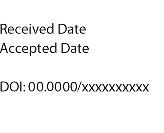
\includegraphics{head_foot/dates} & \\

\end{tabular}

 \end{@twocolumnfalse} \vspace{0.6cm}

  ]
%%%END OF TITLE AND AUTHORS%%%

%%%FONT SETUP - please do not change any commands within this section
\renewcommand*\rmdefault{bch}\normalfont\upshape
\rmfamily
\section*{}
\vspace{-1cm}


%%%FOOTNOTES%%%

\footnotetext{\textit{$^{a}$~Chemical Research Laboratory, South Parks Road, Oxford, OX1 1NQ.}}

%Please use \dag to cite the ESI in the main text of the article.
%If you article does not have ESI please remove the the \dag symbol from the title and the footnotetext below.
\footnotetext{\dag~Electronic Supplementary Information (ESI) available: [details of any supplementary information available should be included here]. See DOI: 00.0000/00000000.}
%additional addresses can be cited as above using the lower-case letters, c, d, e... If all authors are from the same address, no letter is required

% \footnotetext{\ddag~Additional footnotes to the title and authors can be included \textit{e.g.}\ `Present address:' or `These authors contributed equally to this work' as above using the symbols: \ddag, \textsection, and \P. Please place the appropriate symbol next to the author's name and include a \texttt{\textbackslash footnotetext} entry in the the correct place in the list.}

%%%END OF FOOTNOTES%%%

%%%ABSTRACT%%%%

\sffamily{\textbf{The abstract should be a single paragraph which summarises the content of the article.}}\\%The abstrast goes here instead of the text "The abstract should be..."

%%%END OF ABSTRACT%%%%

\rmfamily %Please do not remove this line.

%%%MAIN TEXT%%%%



Simulating chemical reactions is essential to developing fundamental understanding and predicting experimental outcomes.1 Machine learned potentials (MLPs) offer an enticing approach to chemical simulation, enabling the efficient mapping between nuclear configurations and energies ($\boldsymbol{R} \mapsto E$). Moreover, they offer flexibility and systematic improvability, not possible with classical molecular mechanics (MM).2 Propagating quantum dynamics using these forces should afford experimental rate and equilibrium constants in the limit of correct forces and converged sampling. However, despite the development of Gaussian Approximation Potentials (GAPs)3,4 and high dimensional neural network potentials (NNPs)5 more than 10 years ago, they are still not yet routinely used to simulate chemical reactivity.6 Most likely, this is due to the computational and time investment required to train potentials for new systems. 

Training an MLP consists of: (1) developing a training set; (2) hyperparameter optimisation and (3) performing the regression, repeating the process until the desired accuracy is obtained. Automated approaches to training set construction have been developed,7–9 but can be limited to small systems or generate huge datasets. These limitations coupled with the time required to perform hyperparameter optimisation (if the MLP is insufficiently accurate) inhibits quickly accessing bespoke MLPs. Furthermore, the required $\gg 10^3$ reference evaluations precludes using accurate wavefunction-based quantum methods to evaluate energy and forces without considerable investement.10 Exceptions are rare and limited to systems with $<10$ atoms.8,11 

For potentials suitable to simulate chemical reactivity, automated approaches are essential. The energy scale over which the potential must be accurate is larger, necessitating exponentially more training data and thus bespoke MLPs. Furthermore, the complex electronic structure around transition states makes density functional theory (DFT) a poorer reference method,12 meaning coupled-cluster (CC) is often the target surface for quantitative comparison to experiment, which in-turn demands data-efficient strategies.

Here, we show that new MLP regression methods13,14 can be used to generate accurate potentials for modestly sized reactions (~50 atoms) in an automated fashion and demonstrate the associated insights that can be obtained. 

With a view to extend our initial GAP training methodology8 into more complex systems and environments, we considered Diels-Alder (DA) reactions because of the available theoretical and experimental data,15,16 and their prominence in chemical and biochemical contexts.17–19 Initial efforts proved promising, with qualitatively reasonable reaction dynamics from [4+2] cycloaddition TSs for reactions between ethene + butadiene20 (R1) and methyl-vinyl ketone + cyclopentadiene (R2). Evaluating the quality of these potentials, however, revealed that they were not within the few kBT accuracy limit required for rate estimation or dynamic studies (see e.g., Figure S1a). A similarly complex but less exothermic reaction (\ce{H3C}· + \ce{C3H8} $\rightarrow$ \ce{CH4} + ·\ce{CH(CH3)2}) could be trained using the same strategy and hyperparameters (Figure S1b), suggesting that achieving 1 kcal mol–1 accuracy within a 60 kcal mol–1 energy window required for R1 is challenging for a GAP. Hyperparameter optimisation afforded an improvement, but at moderate computational cost (~500 configurations required for R1). Specifically, increasing the ‘strength’ of the fit by reducing the noise added to energies and forces, increasing the quality of the radial basis, and doubling the number of atomic environments considered in the training all improved the GAP (SI §S3). Systematic investigation of the effect of system size on the required number of reference evaluations suggests an approximate exponential scaling for a desired accuracy on the total energy (SI §S2). Adopting new regression methods within the same training strategy (Figure X1) shows that GAPs – even with hyperparameter tuning – are outperformed by both linear atomic cluster expansion (ACE21) and equivariant graph neural networks (NequIP13). While rather different in philosophy, both frameworks provide MLPs that are similarly accurate for R1 (Figure X1a, Figure S?). Here, accuracy is based on deviations between true and predicted energies over independent DFT-MD trajectories propagated from the transition state (TS) to the reactant and product states. Previously, we have shown that a prospective validation strategy in the configuration space accessible to that MLP is essential to characterising ‘good’ MLPs.8 However, here these potentials are ‘stable’ by construction, within their own configuration space over the course of the reaction.


\begin{figure}[h]
\centering
%  \includegraphics[height=3cm]{example1}
  \caption{An example figure.}
  \label{fgr:example}
\end{figure}

%\begin{figure*}
% \centering
% \includegraphics[height=3cm]{example2}
% \caption{An image from the \textit{Physical Chemistry Chemical Physics} cover gallery, set as a double-column figure.}
% \label{fgr:example2col}
%\end{figure*}


%  \ce{H2SO4}. 

\clearpage
The conclusions section should come at the end of article. For the reference section, the style file \texttt{rsc.bst} can be used to generate the correct reference style.\footnote[4]{Footnotes should appear here. These might include comments relevant to but not central to the matter under discussion, limited experimental and spectral data, and crystallographic data.}

\section*{Author Contributions}
X

\section*{Conflicts of interest}
There are no conflicts to declare.



%%%END OF MAIN TEXT%%%

%  For footnotes in the main text of the article please number the footnotes to avoid duplicate symbols. e.g.  \footnote[num]{your text} the corresponding author \ast counts as footnote 1, ESI as footnote 2, e.g. if there is no ESI, please start at [num]=[2], if ESI is cited in the title please start at [num]=[3] etc. Please also cite the ESI within the main body of the text using \dag.

% The \balance command can be used to balance the columns on the final page if desired. It should be placed anywhere within the first column of the last page.

% \balance

% If notes are included in your references you can change the title from 'References' to 'Notes and references' using the following command:
% \renewcommand\refname{Notes and references}

%%%REFERENCES%%%
\scriptsize{
\bibliography{rsc} %You need to replace "rsc" on this line with the name of your .bib file
\bibliographystyle{rsc} } %the RSC's .bst file

\end{document}
